\documentclass[10pt,a4paper]{article}
\usepackage[utf8]{inputenc}
\usepackage[spanish]{babel}
\usepackage{amsmath}
\usepackage{amsfonts}
\usepackage{amssymb}
\usepackage{hyperref}
\usepackage{graphicx}
\usepackage{tabularx}
\usepackage[table,xcdraw]{xcolor}
\usepackage[left=2.5cm,right=2.5cm,top=2.5cm,bottom=2.5cm]{geometry}

\hypersetup{
    colorlinks,
    citecolor=black,
    filecolor=black,
    linkcolor=black,
    urlcolor=black
}

\title{Plan de pruebas}
\author{Canosa Domínguez, Cristofer \\ Rodríguez Alcaraz, Silvia \\ Seijas Salinas, Orquídea Manuela \\ Soutullo Sobral, Samuel}
\date{Ingeniería del Software}

\begin{document}
	\maketitle
	
	\newpage
	\begin{table}[htpb]
		\centering
		\begin{tabular}{|l|l|l|}
			\hline
			\rowcolor[HTML]{9B9B9B} 
			\multicolumn{3}{|c|}{\cellcolor[HTML]{9B9B9B}{\color[HTML]{000000} \textbf{CONTROL DE VERSIONES}}} \\ \hline
			\rowcolor[HTML]{C0C0C0} 
			\textbf{Edición} & \textbf{Fecha} & \textbf{Descripción del cambio} \\ \hline
			1.0 & 02/04/2017 & Diseño y casos de prueba de caja negra \\ \hline
		\end{tabular}
	\end{table}
	
	\newpage
	\tableofcontents
	\newpage
	
\section{Plan de pruebas}
	\subsection{Identificador único del documento}
		\texttt{PDP\_v1}

	\subsection{Introducción}
	%TODO Añadir encabezado
		Este documento se corresponde con el plan de pruebas correspondiente al proyecto de ventas de la USC. El software se basa en un portal web mediante el cual los usuarios pueden solicitar pedidos, siendo tramitados posteriormente por la universidad.

		El objetivo de este plan es marcar las pautas y definir la estrategia que se seguirá para certificar el software. En este caso, los casos de prueba y procedimientos tan sólo están generados mediante métodos de caja negra contra la especificación de las interfaces del software.

		Por tanto, los elementos sobre los que se aplicarán las pruebas son las interfaces correspondientes a los módulos de importación, control, estadística y acceso a base de datos (DAO). Dado que las pruebas son de caja negra, se centrarán en el estudio de las especificaciones: testear las entradas para comprobar si se obtienen las salidas esperadas. Para la selección de casos de prueba se utilizó un enfoque sistemático basado en el método de partición o clases de equivalencia.
	
			\subsubsection{Documentos relacionados}
				\begin{table}[htpb]
					\centering
					\begin{tabular}{|l|l|}
					\hline
					\textbf{Nombre} & \textbf{Descripción} \\ \hline
					02\_PlantAnaDisPlan\_v1.pdf & Documento de análisis y diseño del software. \\ \hline
					Std\_IEEE\_829.pdf & Estándar 829 \\ \hline
					\end{tabular}
				\end{table}

	\subsection{Elementos software a probar}
		Como ya se ha mencionado en la introducción, los elementos a probar son los módulos de importación, estadístico, control y DAO a través de pruebas de caja negra sobre sus interfaces.

	\subsection{Características a probar}
		Dado que son pruebas funcionales, las características de las interfaces a probar son las entradas pertinentes a sus métodos. Se pretende comprobar, mediante una serie de casos de prueba planteados mediante partición, que para una entrada dada se obtiene la salida esperada.

	\subsection{Características que no se prueban}
		Partiendo de que se utilizan pruebas de caja negra, todas las características a nivel estructural del software (caja blanca) no se probarán en esta versión del software. Además, puesto que se ha planteado centrar la búsqueda de errores en las interfaces, no se realizarán pruebas centradas en las funciones incorrectas o ausentes, estructuras de datos o acceso a BBDD, rendimiento o errores de inicialización y terminación.

	\subsection{Enfoque general de la prueba}
		Dada la importancia de los formatos para los distintos atributos expuestos en los requisitos, las pruebas se centraron en asegurar su correcta interpretación. Para ello se utilizó principalmente el método de partición para crear casos de prueba.

		Como segunda técnica se usó el análisis por valores límite y, con menor frecuencia, la conjetura de errores.

		Teniendo en cuenta que las pruebas se centran en generación de clases del modelo, muchos de los métodos se consideraron similares entre sí, asumiendo que si uno de ellos es correcto sería apropiado pensar que el resto también lo serán. Sin embargo, atendiendo al teorema de Pareto, en el caso de que uno de estos métodos falle, será conveniente ampliar los casos de prueba a todos sus métodos similares.

	\subsection{Criterios de paso/fallo para cada elemento}
		La aprobación o rechazo de un elemento sobre el que se han aplicado pruebas se basará en un criterio basado en gravedad de errores. El elemento podrá ser aprobado si se han realizado el 100\% de pruebas sobre él y ha obtenido un 90\% de éxito. El 10\% se correspondería a errores medios y leves, pero nunca graves. Un elemento que contenga errores graves, aunque sólo sea uno, no podrá ser aprobado. A continuación, se especifica qué se entiende por error leve, medio y grave:
		
		\begin{itemize}
			\item \textbf{Error leve:} el elemento muestra un comportamiento correcto, pero ligeramente variable en situaciones similares. También se entienden como errores leves pequeñas desviaciones con respecto a los estándares a seguir.
			
			\item \textbf{Error medio:} es un error medio el hecho de que los métodos del elemento a probar, pese a funcionar, realicen sus operaciones de manera incorrecta o no de la forma previamente planteada. En otras palabras, que el elemento no cumpla los requisitos que se le habían impuesto pese a su aparente buen funcionamiento.
			
			\item \textbf{Error grave:} el elemento no cumple el objetivo para el que fue diseñado. También se considera error grave cuando la salida de un método del elemento provoca una situación inesperada y no controlada.
		\end{itemize}

	\subsection{Criterios de suspensión y requisitos de reanudación}
		En ocasiones cuando el número o tipo de errores llega a un punto en el que el seguimiento de la prueba no tiene valor, es mejor barajar el hecho de frenar el proceso de pruebas. A continuación, se indican las situaciones en las que se frenaría dicho proceso con el fin de no desperdiciar recursos:
		
		\begin{itemize}
			\item \textbf{Existencia de un error grave:} una vez se encuentra un error grave en un elemento a probar dentro de un caso de prueba, lo mejor es frenar dicha prueba dado que, como ya se ha mencionado, no es posible que vaya a aprobar. En este caso, el elemento deberá ser estudiado y depurado con el fin de remediar dicho error y continuar con las pruebas más adelante.
			
			No dejando pasar errores críticos se evita el confundir errores fantasma provocados por este error con meros defectos.
			
			\item \textbf{Ningún elemento está preparado para ser probado:} en este caso, realizar pruebas sobre elementos que todavía se encuentran en un estado prematuro sólo conseguirá desperdiciar recursos y no obtener ningún tipo de información esclarecedora. Lo mejor en este caso, es dejar pasar un período de tiempo donde se complementen los elementos y, en este punto, realizar sobre ellos las pruebas.
			
			\item \textbf{Se supera un 20\% de errores al probar un elemento:} aunque sean errores leves o medios, un elemento con un 20\% de errores acabará provocando más fallos en el conjunto de la aplicación en algún momento. De alcanzar y superar este límite, este elemento debe ser revisado para poder volver a realizar pruebas sobre él en un futuro. 
			
			\item \textbf{No disponibilidad del software apropiado para realizar las pruebas:} si las pruebas han sido planteadas para realizar de una forma concreta es mejor esperar a tener todas las herramientas disponibles. Sustituir estas herramientas por otras puede provocar una pérdida de tiempo posterior o el rediseño de alguna prueba.
		\end{itemize}

	\subsection{Documentos a entregar}
		Puesto que en este punto tan sólo se ha planteado la aplicación de pruebas de caja negra, los documentos a entregar tras la realización de las pruebas serían:
		
		\begin{itemize}
			\item Informe de pruebas de caja negra.
			\item Código de los elementos a probar
			\item Código de las pruebas que se realizaron
		\end{itemize}

	\subsection{Actividades de preparación y ejecución de pruebas}
		Para el correcto desarrollo de las pruebas se necesita contar con equipos que contengan el software que se utilizará para su realización. En este caso, \emph{Mockito} y \emph{JUnit}, además del correspondiente \emph{IDE} de trabajo que compartirán todos los programadores de pruebas a la hora de codificar: \emph{Eclipse}. Es obvio que, además, todo el personal implicado en la ejecución de las pruebas tendrá acceso al código de las implementado, el código de los elementos a probar y el plan de pruebas a seguir.

	\subsection{Necesidades de entorno}
		Para la realización de las pruebas será necesario tener una base de datos funcional con los datos necesarios para cada uno de los casos de prueba. Dado que los casos serán idempotentes siempre que no se indique lo contrario, serán ellos los encargados de inicializar la base de datos a sus valores necesarios para la correcta ejecución.

	\subsection{Responsabilidades en la organización y realización de las pruebas}
		Para la realización de las pruebas se precisará un equipo de pruebas que podría estar formado por personas que cumplan los siguientes roles (entiéndase que sólo existiría un jefe de proyecto):
		
		\begin{table}[]
\centering
\begin{tabularx}{\textwidth}{|l|X|}
\hline
\textbf{Rol}           & \textbf{Responsabilidad}                                                                                                                                                                                               \\ \hline
Jefe de proyecto       & Responsable de estudiar las condiciones de finalización del proceso de pruebas. Será tarea suya concluir si el producto probado está listo o no. También es su deber coordinar al resto del equipo y delegar sobre él. \\ \hline
Analista               & Persona encargada de resolver las incidencias, analizar los resultados y generar los informes correspondientes para comunicar los resultados técnicos al jefe de proyecto.                                             \\ \hline
Programador de pruebas & Responsable de la generación del plan de pruebas.                                                                                                                                                                      \\ \hline
\end{tabularx}
\end{table}

	\subsection{Necesidades de personal y de formación}
		Por una parte, el personal debe poseer los conocimientos técnicos informáticos suficientes como para poder implementar las pruebas que se van a realizar y comprender el código a probar, además de saber manejar las herramientas planteadas para el desarrollo de las pruebas.

		Por otra parte, es necesaria una figura que lidere el equipo de pruebas y coordine a todos sus integrantes, con capacidad de liderazgo. Sus conocimientos estarían más orientados a la empresa pese a que sería apropiado que tuviese implicación dentro de las TICs.

		Finalmente, sería necesaria una persona centrada en el análisis e interpretación de los resultados obtenidos en las pruebas, que comunicase el equipo de testing con el jefe de proyecto. Sería conveniente que esta persona tuviese conocimientos en el área de la ingeniería y, como requisito recomendable, experiencia previa.


	\subsection{Esquema de tiempos}
		\begin{figure}[htpb]
			\centering
			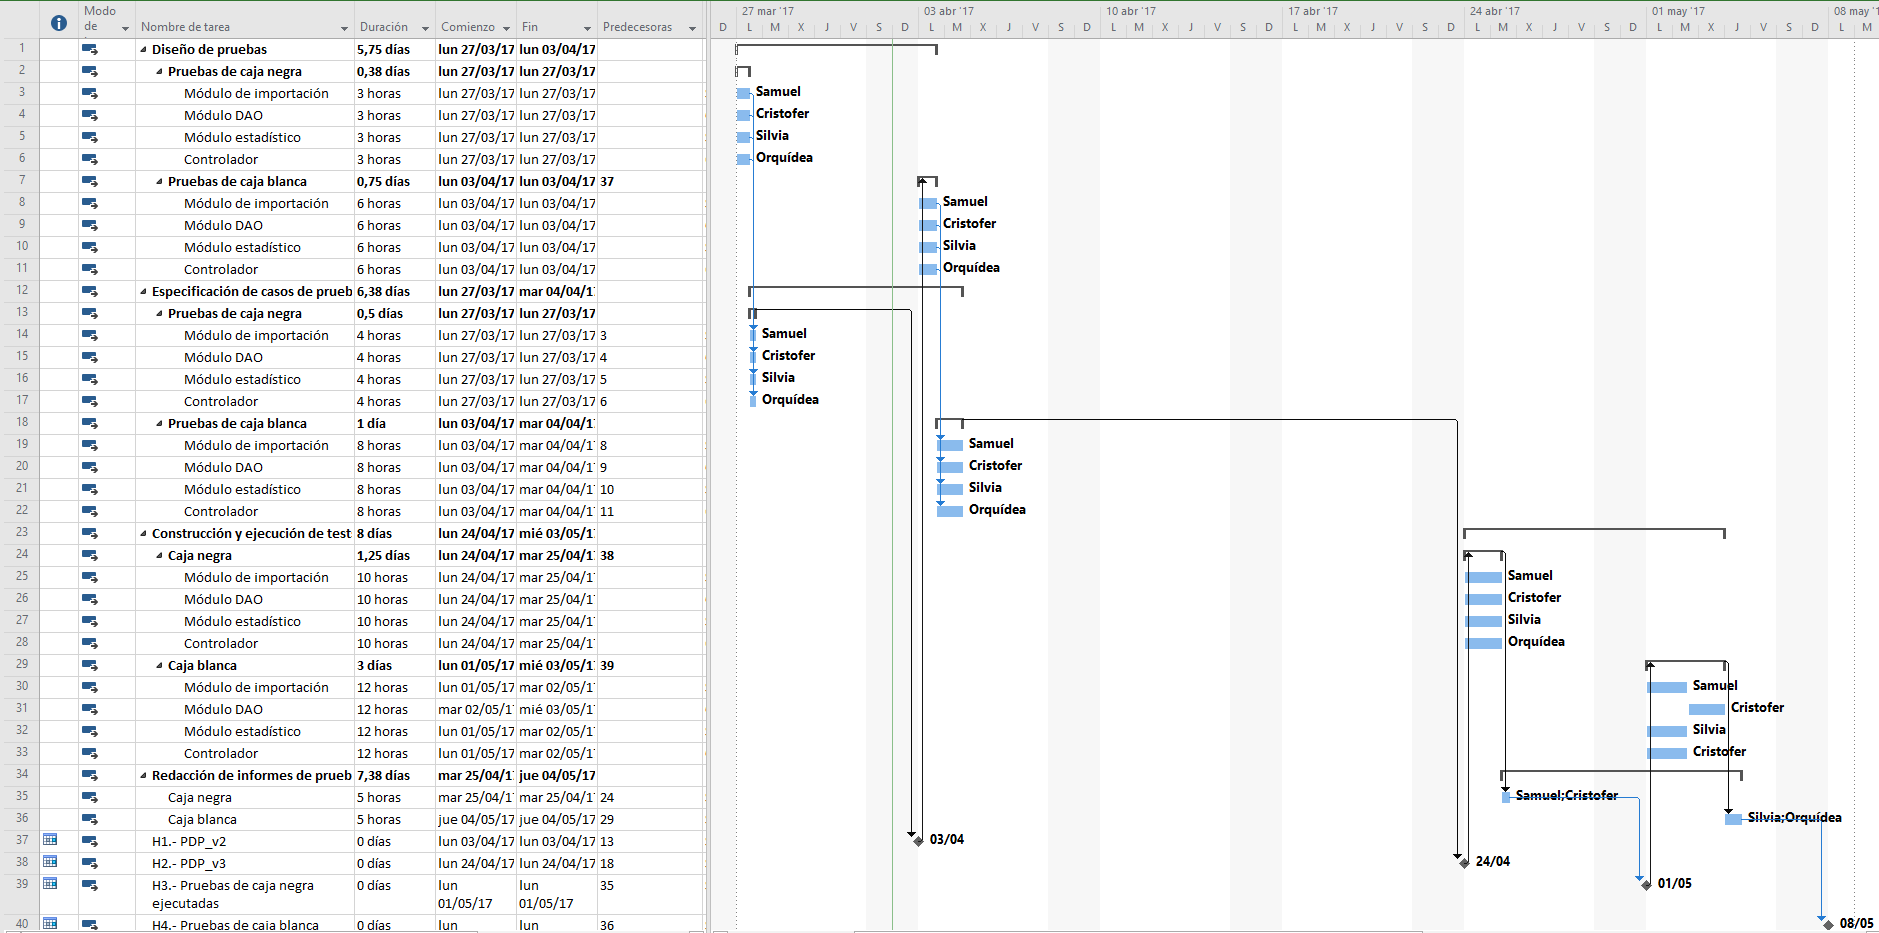
\includegraphics[width=\textwidth]{../anexos/PlanDePruebas.PNG}
			\caption{Diagrama de Gantt}
			\label{fig:gantt}
		\end{figure} 

	\subsection{Riesgos asumidos por el plan y planes de contingencias para cada riesgo}
		\begin{table}[htpb]
			\centering
			\label{my-label}
			\begin{tabularx}{\textwidth}{|X|X|X|}
				\hline
				\textbf{Riesgo}                                                  & \textbf{Descripción}                                                       & \textbf{Contigencia}                                                                                  \\ \hline
				Fuerte limitación temporal para el planteamiento de las pruebas. & Intervalo de tiempo escaso para diseñar el plan de pruebas.                & Generación de pruebas de caja negra sin excesivo nivel de detalle para cumplir las fechas de entrega. \\ \hline
				Cambios en los requisitos o diseños originales.                  & Incoherencias y falta de información en el documento de análisis y diseño. & Diálogo intergrupal para solucionar posibles malas interpretaciones.                                  \\ \hline
				Recursos con escaso tiempo para asignar a las pruebas.           & Recursos con poca disponibilidad.                                          & Redistribución de la carga entre recursos más disponibles.                                            \\ \hline
			\end{tabularx}
		\end{table}

	\subsection{Aprobaciones y firmas con nombre y puesto desempeñado}
		La aprobación para definir el proceso como completo y permitir que avance al siguiente nivel es una tarea cooperativa entre dos departamentos. Mediante una reunión formal en la que se encuentren el jefe de desarrollo y el analista a cargo del proyecto se decidirá si el software está preparado. Se precisa de la aprobación de ambos ya que es necesario contar con un aprobado a nivel técnico y otro más enfocado a un nivel empresarial. De esta forma, mediante el debate y el estudio de los informes de pruebas se considera que el software pasa a la siguiente fase si se aprueba por unanimidad.

		La firma del analista y el jefe de desarrollo supondrían la aprobación del software y, por tanto, el pase a la siguiente fase del proyecto.


\section{Diseño de pruebas}
	\subsection{InterfazImportación}
			\subsubsection{Prueba I-01}
			\paragraph{Objetivo} Comprobar que un archivo con líneas incompletas, con demasiados campos, o en blanco no provoca un comportamiento inesperado en el programa.
			\paragraph{Técnicas de caja negra} Aplicando las reglas especificadas a continuación se obtienen las siguientes clases de equivalencia:
			\begin{itemize}
				\item \textbf{R1:} incluir una línea con campos de menos (todos ellos con valores válidos), otra línea con campos de más (los que no se hayan incluido a mayores deben tener valores válidos) y una línea con el número de campos correctos (todos ellos con valores válidos).
				\item \textbf{R3:} incluir una línea en blanco y otra completa y correcta.
			\end{itemize}
			Dado que las clases de equivalencia se obtienen en base al contenido del archivo, se aplicarán a los tres métodos de la interfaz  (\textit{importarUsuarios}, \textit{importarProducto} e \textit{importarCompra}).
			\paragraph{Criterios de paso/fallo}
			En ninguno de los casos se debe generar una excepción no controlada como consecuencia del formato inesperado de la línea del fichero. Cuando un archivo contenga líneas incorrectas se debe cancelar la importación informando al usuario del error. Por otra parte, un archivo con líneas correctas debe ser correctamente procesado.
			\paragraph{Resultado de aplicar las ténicas}
%TODO Añadir tabla de resultado			
			\subsubsection{Prueba I-02}
			\paragraph{Objetivo} Comprobar que un archivo que contenga un campo con un formato o valor incorrecto no provoca un comportamiento inesperado en el programa.
			\paragraph{Técnicas de caja negra} Aplicando las reglas especificadas a continuación se obtienen las siguientes clases de equivalencia:
			\begin{itemize}
				\item \textbf{R1:} para todos los campos con longitud máxima delimitada, se probará introduciendo el campo vacío, el campo con una longitud correcta, y el campo con una longitud superior a la correcta.
				\item \textbf{R3:} para cada uno de los campos sujetos a restricción de formato, se probará un caso con formato correcto y otro con formato incorrecto (por ejemplo: fecha con formato adecuado, unidades, cantidad y precio deben ser numéricos, etc.).
				\item \textbf{R3:} para cada uno de los campos identificadores, se probará un caso con un identificador ya presente en la base de datos, y otro no presente en la base de datos. En otras palabras, se probará a importar un elemento ya presente en la base de datos y otro que no lo esté.
				\item \textbf{R3:} para los campos de referencia a ítem y usuario en las líneas de venta, se probará un caso en el que el identificador del ítem o usuario referenciado se encuentre previamente en la base de datos y otro caso en el que no.
			\end{itemize}
			Dado que las clases de equivalencia se obtienen en base al contenido del archivo, se aplicarán a los tres métodos de la interfaz  (\textit{importarUsuarios}, \textit{importarProducto} e \textit{importarCompra}).
			
			Dada su relación directa con el tipo de línea en cuestión, las reglas que se listan a continuación sí se aplican de manera diferente a cada método:
			\begin{itemize}
				\item \textbf{\textit{importarUsuarios}}
					\begin{itemize}
						\item \textbf{R3:} un caso en el que el primer campo sea \textit{U} y otro en el que sea distinto de \textit{U}.
					\end{itemize}
				\item \textbf{\textit{importarProducto}}
					\begin{itemize}
						\item \textbf{R3:} un caso en el que el primer campo sea \textit{I} y otro en el que sea distinto de \textit{I}.
					\end{itemize}
				\item \textbf{\textit{importarCompra}}
					\begin{itemize}
						\item \textbf{R3:} un caso en el que el primer campo sea \textit{V} y otro en el que sea distinto de \textit{V}.
					\end{itemize}
			\end{itemize}
			Aplicando las técnicas de análisis por valores límite se obtiene lo siguiente:
			\begin{itemize}
				\item \textbf{R1:} para todos los campos con longitud máxima \textit{m}, se probará introduciendo valores con longitud 0, \textit{m} y \textit{m+1}.
			\end{itemize}
			Finalmente, aplicando la técnica de conjetura de errores, se obtiene lo siguiente:
			\begin{itemize}
				\item Se debe comprobar si la existencia de varias líneas de venta con el mismo identificador provoca que se añadan varios ítems a la misma venta. Si esto no sucede, el comportamiento es incorrecto.
			\end{itemize}
			\paragraph{Criterios de paso/fallo}
	En ninguno de los casos se debe generar una excepción no controlada como consecuencia del formato o valor inesperado del campo. Cuando un archivo contenga uno o más campos incorrectos se debe cancelar la importación informando al usuario del error. Por otra parte, un archivo con todos los campos correctos debe ser correctamente procesado.
			\paragraph{Resultado de aplicar las ténicas}
			%TODO Añadir tabla resultado de aplicar las técnicas
			\subsubsection{Prueba I-03}
			\paragraph{Objetivo}
			\paragraph{Técnicas de caja negra}
			\paragraph{Criterios de paso/fallo}
			\paragraph{Resultado de aplicar las ténicas}
	\subsection{InterfazDAO}
			\subsubsection{Prueba D-01}
			\paragraph{Objetivo} Comprobar que las inserciones o modificaciones de usuarios se reflejan correctamente en la base de datos.
			Además, se busca que, en caso de error, este sea correctamente gestionado.
			\paragraph{Técnicas de caja negra} Centrándose en los métodos de inserción y modificación de usuarios y haciendo uso de las reglas especificadas, se definen las siguientes clases:
			\begin{itemize}
				\item \textbf{\textit{Insertar usuario}}
					\begin{itemize}
						\item \textbf{R3:} Probar un usuario con ID válido y otro sin ID.
						\item \textbf{R5:} Los ID de usuario de forma N-XXXXXX-000:
							\begin{itemize}
								\item \textit{R1:} Cadena de letras con 5 y 7 caracteres (incorrecto) y una correcta. Clase equivalente para la cadena numérica.
								\item \textit{R3:} Eliminar uno de los campos del ID.
								\item \textit{R3:} Que N sea U u otro caracter.
							\end{itemize}
					\end{itemize}
				\item \textbf{\textit{Modificar usuario}}
					\begin{itemize}
						\item Se supone que la introducción del usuario modificado en la base de datos será equivalente a la usada en el método anterior y, por tanto, ya está probada.
						\item \textbf{R3: } Insertar datos modificados de un usuario existente (caso correcto) e insertar datos de un usuario que no existe.
					\end{itemize}
			\end{itemize}
			\paragraph{Criterios de paso/fallo} Los usuarios introducidos o modificados usando datos correctos deben verse reflejados en la base de datos.
			En los casos de incluir usuarios de forma errónea debe notificarse del error y en ningún caso reflejarse en la base de datos.
			\paragraph{Resultado de aplicar las ténicas}
			\subsubsection{Prueba D-02}
			\paragraph{Objetivo} Comprobar que las inserciones o modificaciones de items y ventas se reflejan correctamente en la base de datos.
			Además, se busca que, en caso de error, este sea correctamente gestionado.
			Dada su similitud con las pruebas para usuarios no se hará una prueba exhaustiva excepto en el caso de que se encuentren fallos en las pruebas anteriores.
			\paragraph{Técnicas de caja negra} Centrándose en los métodos de inserción y modificación de items y ventas, y haciendo uso de las reglas especificadas, se definen las siguientes clases:
			\begin{itemize}
				\item \textbf{\textit{Insertar item / venta / Modificar item}}
					\begin{itemize}
						\item \textbf{R3:} Id válido para la inserción y uno inválido.
						\item \textbf{R3:} Id existente y no existente para la modificación.
					\end{itemize}
			\end{itemize}
			\paragraph{Criterios de paso/fallo} Los items o ventas introducidos o modificados usando datos correctos deben verse reflejados en la base de datos.
			En los casos de incluir items o ventas de forma errónea debe notificarse del error y en ningún caso reflejarse en la base de datos.
			\paragraph{Resultado de aplicar las ténicas}
			\subsubsection{Prueba D-03}
			%TODO revisar: el método isLoged ya no existe, ahora hay logIn y está en el controlador.
			\paragraph{Objetivo}
			\paragraph{Técnicas de caja negra}
			\paragraph{Criterios de paso/fallo}
			\paragraph{Resultado de aplicar las ténicas}
			\subsubsection{Prueba D-04}
			%TODO validar pedido ya no recibe lo mismo que antes
			\paragraph{Objetivo}
			\paragraph{Técnicas de caja negra}
			\paragraph{Criterios de paso/fallo}
			\paragraph{Resultado de aplicar las ténicas}
			\subsubsection{Prueba D-05}
			%TODO getHistorialUsuario ya no recibe un string.
			\paragraph{Objetivo}
			\paragraph{Técnicas de caja negra}
			\paragraph{Criterios de paso/fallo}
			\paragraph{Resultado de aplicar las ténicas}
	\subsection{InterfazEstadistica}
			\subsubsection{Prueba E-01}
			\paragraph{Objetivo} Comprobar que para entradas incorrectas en los métodos de la interfaz no se producen situaciones no controladas o inesperadas.
			\paragraph{Técnicas de caja negra} Se ha aplicado la siguiente regla a todos los métodos de la interfaz ya que todos reciben la misma entrada: un entero en el rango [1,3] para referenciar respectivamente a días, semanas y meses.
			\begin{itemize}
				\item \textbf{\textit{getValoresBrutos / getMedias / getHistos / getPorcentajes}}
					\begin{itemize}
						\item \textbf{R4:} Introducir cada uno de los modos correctos {1,2,3} y uno incorrecto.
					\end{itemize}
			\end{itemize}
			\paragraph{Criterios de paso/fallo} Dada una entrada no esperada de un método, ésta no puede provocar un comportamiento no controlado. De ocurrir esto, la consulta realizada se omitirá, devolviendo un mensaje de error indicando que el método no se ha utilizado de manera apropiada.
			\paragraph{Resultado de aplicar las ténicas}
	\subsection{InterfazControlador}
			\subsubsection{Nota}

			\subsubsection{Prueba C-01}
			\paragraph{Objetivo}
			\paragraph{Técnicas de caja negra}
			\paragraph{Criterios de paso/fallo}
			\paragraph{Resultado de aplicar las ténicas}
			\subsubsection{Prueba C-02}
			%TODO ya no hay insercion de compras, sino de orders.
			\paragraph{Objetivo}
			\paragraph{Técnicas de caja negra}
			\paragraph{Criterios de paso/fallo}
			\paragraph{Resultado de aplicar las ténicas}
			\subsubsection{Prueba C-03}
			%TODO revisar porque ahora hay orders
			\paragraph{Objetivo}
			\paragraph{Técnicas de caja negra}
			\paragraph{Criterios de paso/fallo}
			\paragraph{Resultado de aplicar las ténicas}
			\subsubsection{Prueba C-04}
			\paragraph{Objetivo}
			\paragraph{Técnicas de caja negra}
			\paragraph{Criterios de paso/fallo}
			\paragraph{Resultado de aplicar las ténicas}
			\subsubsection{Prueba C-05}
			\paragraph{Objetivo}
			\paragraph{Técnicas de caja negra}
			\paragraph{Criterios de paso/fallo}
			\paragraph{Resultado de aplicar las ténicas}
\section{Casos de prueba}
	\subsection{InterfazImportacion}
			\subsubsection{Caso de prueba I-01-P-01}
			\paragraph{Contexto de ejecución}
			\paragraph{Definición}
			\paragraph{Clases que valida}
			\paragraph{Resultado esperado}

			\subsubsection{Caso de prueba I-01-P-02}

			\subsubsection{Caso de prueba I-01-P-03}

			\subsubsection{Caso de prueba I-01-P-04}

			\subsubsection{Caso de prueba I-02-P-01}

			\subsubsection{Caso de prueba I-02-P-02}

			\subsubsection{Caso de prueba I-02-P-03}

			\subsubsection{Caso de prueba I-02-P-04}

			\subsubsection{Caso de prueba I-02-P-05}

			\subsubsection{Caso de prueba I-02-P-06}

			\subsubsection{Caso de prueba I-02-P-07}

			\subsubsection{Caso de prueba I-02-P-08}

			\subsubsection{Caso de prueba I-02-P-09}

			\subsubsection{Caso de prueba I-02-P-10}

			\subsubsection{Caso de prueba I-03-P-01}

			\subsubsection{Caso de prueba I-03-P-02}

			\subsubsection{Caso de prueba I-03-P-03}

	\subsection{InterfazDAO}
			\subsubsection{Caso de prueba D-01-P-01}
				\paragraph{Contexto de ejecución} Valida la inserción correcta de un usuario.
				\paragraph{Definición}
				\begin{itemize}
					\item \textit{Usuario:}
					\begin{itemize}
						\item \textbar  U-abcdef-000 \textbar Manuel \textbar Soutoullo \textbar 10-10-2010 \textbar alumno \textbar
					\end{itemize}
				\end{itemize}
				\paragraph{Clases que valida} 1, 3, 6, 9, 10.
				\paragraph{Resultado esperado} Inserción del usuario con id: U-abcdef-000 en la base de datos.
			\subsubsection{Caso de prueba D-01-P-02}
				\paragraph{Contexto de ejecución} Valida la inserción correcta de un usuario.
				\paragraph{Definición}
				\begin{itemize}
					\item \textit{Usuario:}
					\begin{itemize}
						\item \textbar x \textbar Manuel \textbar Soutoullo \textbar 10-10-2010 \textbar alumno \textbar
					\end{itemize}
				\end{itemize}
				\paragraph{Clases que valida} 2.
				\paragraph{Resultado esperado} Notificación de error por parte de la aplicación. Sin consecuencias en la base de datos.
			\subsubsection{Caso de prueba D-01-P-03}
			\paragraph{Contexto de ejecución} Valida la inserción correcta de un usuario.
				\paragraph{Definición}
				\begin{itemize}
					\item \textit{Usuario:}
					\begin{itemize}
						\item \textbar U-abcde-000 \textbar Manuel \textbar Soutoullo \textbar 10-10-2010 \textbar alumno \textbar
					\end{itemize}
				\end{itemize}
				\paragraph{Clases que valida} 4.
				\paragraph{Resultado esperado} Notificación de error por parte de la aplicación. Sin consecuencias en la base de datos.
			\subsubsection{Caso de prueba D-01-P-04}
			\paragraph{Contexto de ejecución} Valida la inserción correcta de un usuario.
				\paragraph{Definición}
				\begin{itemize}
					\item \textit{Usuario:}
					\begin{itemize}
						\item \textbar U-abcdef-0000 \textbar Manuel \textbar Soutoullo \textbar 10-10-2010 \textbar alumno \textbar
					\end{itemize}
				\end{itemize}
				\paragraph{Clases que valida} 8.
				\paragraph{Resultado esperado} Notificación de error por parte de la aplicación. Sin consecuencias en la base de datos.
			\subsubsection{Caso de prueba D-01-P-05}
			\paragraph{Contexto de ejecución} Valida la inserción correcta de un usuario.
				\paragraph{Definición}
				\begin{itemize}
					\item \textit{Usuario:}
					\begin{itemize}
						\item \textbar U-abcdef- \textbar Manuel \textbar Soutoullo \textbar 10-10-2010 \textbar alumno \textbar
					\end{itemize}
				\end{itemize}
				%TODO creo que esto es uno de los errores
				\paragraph{Clases que valida} 10.
				\paragraph{Resultado esperado} Notificación de error por parte de la aplicación. Sin consecuencias en la base de datos.
			\subsubsection{Caso de prueba D-01-P-06}
			\paragraph{Contexto de ejecución} Valida la modificación correcta de un usuario. Se supone que la base de datos solo cuenta con el usuario \textbar U-aaaaaa-000" \textbar Limón Novoa \textbar 10-10-2010 \textbar estudiante \textbar
				\paragraph{Definición}
				\begin{itemize}
					\item \textit{Usuario:}
					\begin{itemize}
						\item \textbar U-aaaaaa-000 \textbar Manuel \textbar Soutoullo \textbar 10-10-2010 \textbar alumno \textbar
					\end{itemize}
				\end{itemize}
				\paragraph{Clases que valida} 12.
				\paragraph{Resultado esperado} En la base de datos el usuario cuyo id es U-aaaaaa-000 pasa a tener el nombre Manuel Soutoullo.

			\subsubsection{Caso de prueba D-01-P-07}
			\paragraph{Contexto de ejecución} Valida la modificación correcta de un usuario. Se supone que la base de datos solo cuenta con el usuario \textbar U-aaaaaa-000" \textbar Limón Novoa \textbar 10-10-2010 \textbar estudiante \textbar
				\paragraph{Definición}
				\begin{itemize}
					\item \textit{Usuario:}
					\begin{itemize}
						\item \textbar U-dddddd-111 \textbar Manuel \textbar Soutoullo \textbar 10-10-2010 \textbar alumno \textbar
					\end{itemize}
				\end{itemize}
				\paragraph{Clases que valida} 13.
				\paragraph{Resultado esperado} Se debe indicar que el usuario no existe y, por tanto, no se puede modificar. Alternativamente puede decidir insertar el nuevo usuario en la base.

			\subsubsection{Caso de prueba D-02-P-01}

			\subsubsection{Caso de prueba D-02-P-02}

			\subsubsection{Caso de prueba D-02-P-03}

			\subsubsection{Caso de prueba D-02-P-04}

			\subsubsection{Caso de prueba D-02-P-05}

			\subsubsection{Caso de prueba D-02-P-06}

			\subsubsection{Caso de prueba D-03-P-01}

			\subsubsection{Caso de prueba D-03-P-02}

			\subsubsection{Caso de prueba D-03-P-03}

			\subsubsection{Caso de prueba D-04-P-01}

			\subsubsection{Caso de prueba D-04-P-02}

			\subsubsection{Caso de prueba D-04-P-03}

			\subsubsection{Caso de prueba D-04-P-04}

			\subsubsection{Caso de prueba D-05-P-01}

			\subsubsection{Caso de prueba D-05-P-02}

			\subsubsection{Caso de prueba D-05-P-03}

			\subsubsection{Caso de prueba D-05-P-04}

	\subsection{InterfazEstadistica}
			\subsubsection{Nota}

			\subsubsection{Caso de prueba E-01-P-01}

			\subsubsection{Caso de prueba E-01-P-02}

			\subsubsection{Caso de prueba E-01-P-03}

			\subsubsection{Caso de prueba E-01-P-04}

	\subsection{InterfazControlador}
			\subsubsection{Caso de prueba C-01-P-01}

			\subsubsection{Caso de prueba C-01-P-02}

			\subsubsection{Caso de prueba C-01-P-03}

			\subsubsection{Caso de prueba C-01-P-04}

			\subsubsection{Caso de prueba C-01-P-05}

			\subsubsection{Caso de prueba C-02-P-01}

			\subsubsection{Caso de prueba C-02-P-02}

			\subsubsection{Caso de prueba C-03-P-01}

			\subsubsection{Caso de prueba C-03-P-02}

			\subsubsection{Caso de prueba C-03-P-03}

			\subsubsection{Caso de prueba C-04-P-01}

			\subsubsection{Caso de prueba C-04-P-02}

			\subsubsection{Caso de prueba C-05-P-01}

			\subsubsection{Caso de prueba C-05-P-02}

\section{Procedimientos de prueba}

\section{Anexo: Plantillas}
	\subsection{Plantilla de plan de pruebas}

	\subsection{Plantilla de diseño de pruebas}

	\subsection{Plantilla de casos de prueba}

	
\end{document}